\documentclass[aspectratio=169,11pt]{ctexbeamer}

\usetheme{Madrid}
\usecolortheme{seahorse}
\setbeamertemplate{navigation symbols}{}
\setbeamertemplate{footline}[frame number]

\usepackage{graphicx}
\usepackage{booktabs}
\usepackage{amsmath}
\usepackage{hyperref}

\graphicspath{{assets/}}

\title{面向不连续地形的 G1 12DoF 感知行走训练}
\subtitle{校级科研项目 5 分钟汇报大纲}
\author{汇报人：\underline{\hspace{3cm}}}
\institute{单位：\underline{\hspace{4cm}}}
\date{\today}

\begin{document}

\begin{frame}
  \titlepage
  \vspace{-0.4em}
  \begin{block}{一句话概括}
    基于 MJLab / MuJoCo Warp / PPO，为 Unitree G1 12DoF 下肢模型训练能感知楼梯、不连续地形并保持自然交替步态的行走策略。
  \end{block}
  \vfill
  {\footnotesize 建议用时：20 秒}
\end{frame}

\begin{frame}{汇报结构}
  \begin{columns}[T,onlytextwidth]
    \column{0.52\textwidth}
    \begin{enumerate}
      \item 研究目标：从“能动”到“像人一样走”
      \item 技术路线：仿真、感知、强化学习
      \item 实现难点：奖励漏洞与训练崩溃
      \item 核心设计：环境课程与奖励函数
      \item 创新点与结果展示
    \end{enumerate}

    \column{0.42\textwidth}
    \begin{block}{展示重点}
      \begin{itemize}
        \item 交替迈步
        \item 不交叉、不跳跃
        \item 上下楼梯保持直走
        \item 脚部抬升高度与身体姿态
      \end{itemize}
    \end{block}
  \end{columns}
  \vfill
  {\footnotesize 建议用时：20 秒}
\end{frame}

\begin{frame}{研究目标与问题定义}
  \begin{columns}[T,onlytextwidth]
    \column{0.54\textwidth}
    \begin{block}{目标}
      在离散、不连续地形中训练 G1 12DoF 下肢模型完成稳定前向行走：
      \begin{itemize}
        \item 两脚交替迈步，脚不能交叉
        \item 膝盖微屈，脚掌稳定落地
        \item 感知前方台阶，不绕开、不侧偏
        \item 从 12cm 台阶扩展到 13.5cm，继续向 15cm 过渡
      \end{itemize}
    \end{block}

    \column{0.42\textwidth}
    \begin{block}{为什么难}
      人形机器人会利用奖励漏洞：
      \begin{itemize}
        \item 单脚跳、拖脚、蹬地
        \item 侧向绕开楼梯
        \item 交叉腿但仍向前移动
        \item 高台阶阶段容易训成跳跃
      \end{itemize}
    \end{block}
  \end{columns}
  \vfill
  {\footnotesize 建议用时：35 秒}
\end{frame}

\begin{frame}{技术路线：感知行走训练闭环}
  \begin{columns}[T,onlytextwidth]
    \column{0.52\textwidth}
    \begin{block}{训练框架}
      \begin{itemize}
        \item 仿真：MJLab + MuJoCo Warp
        \item 算法：RSL-RL PPO
        \item 策略网络：MLP Actor-Critic
        \item 动作空间：12 个关节位置控制
      \end{itemize}
    \end{block}

    \begin{block}{观测信息}
      \begin{itemize}
        \item 本体状态：速度、姿态、关节状态
        \item 地形感知：前方高度扫描 \texttt{height\_scan}
        \item critic 额外输入：脚高、接触、接触力
      \end{itemize}
    \end{block}

    \column{0.42\textwidth}
    \begin{block}{训练流程}
      \[
      o_t \rightarrow \pi_\theta(a_t|o_t)
      \rightarrow \text{MuJoCo step}
      \rightarrow r_t, o_{t+1}
      \]
      \vspace{-0.3em}
      \begin{itemize}
        \item 多环境并行训练
        \item 地形课程逐步提高难度
        \item 看到好模型立即保存为回滚点
      \end{itemize}
    \end{block}
  \end{columns}
  \vfill
  {\footnotesize 建议用时：35 秒}
\end{frame}

\begin{frame}{环境设计：从课程训练到随机展示}
  \begin{columns}[T,onlytextwidth]
    \column{0.46\textwidth}
    \begin{block}{训练地形课程}
      \begin{tabular}{lcc}
        \toprule
        地形 & 比例 & 高度 \\
        \midrule
        平地 & 0.44 & 0 \\
        低上楼梯 & 0.18 & 2--8cm \\
        低下楼梯 & 0.12 & 2--8cm \\
        中上楼梯 & 0.18 & 8.5--13.5cm \\
        中下楼梯 & 0.08 & 6--11.5cm \\
        \bottomrule
      \end{tabular}
    \end{block}

    \begin{block}{几何约束}
      \[
      H_{\text{foot target}} \ge H_{\text{stair max}} + 3\text{--}5cm
      \]
      当前阶段：13.5cm 台阶，18cm 抬脚目标。
    \end{block}

    \column{0.50\textwidth}
    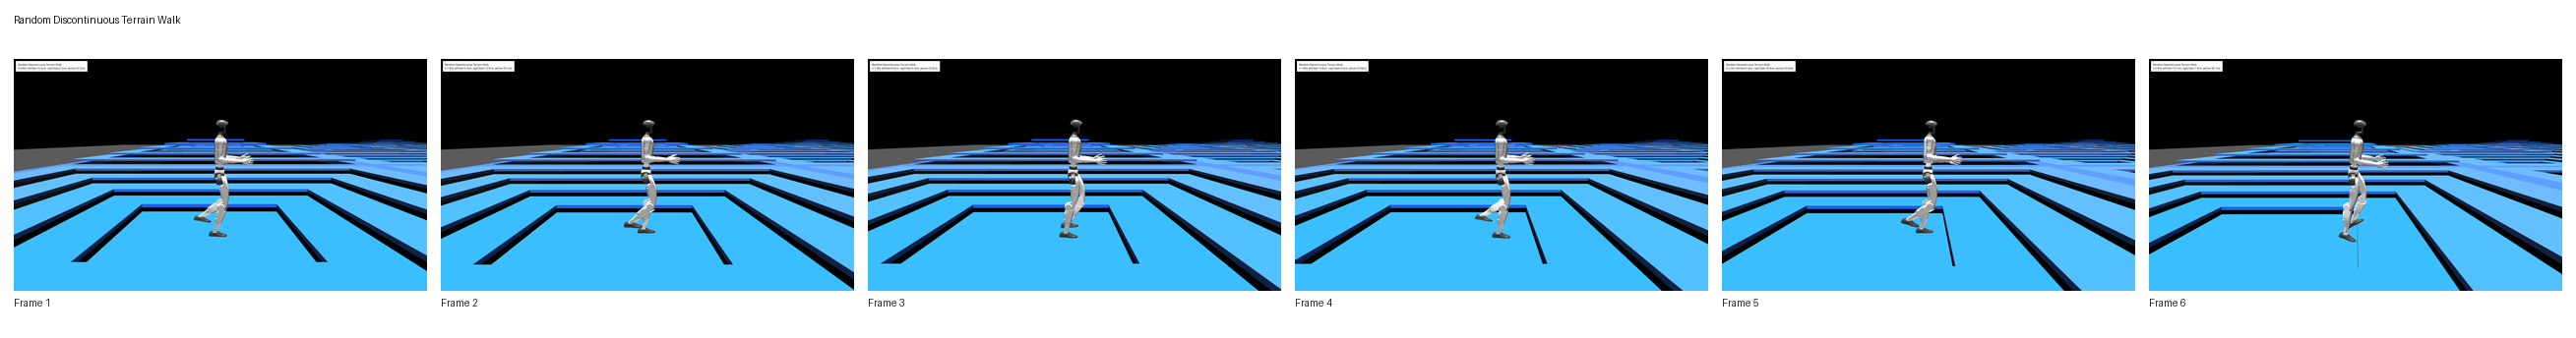
\includegraphics[width=\linewidth]{mixed_contact_sheet.png}
    \vspace{0.3em}
    {\footnotesize 展示模式采用随机不连续地形：随时可能上楼、下楼或进入不规则台阶。}
  \end{columns}
  \vfill
  {\footnotesize 建议用时：45 秒}
\end{frame}

\begin{frame}{奖励函数设计：约束“怎样走”}
  \small
  \begin{columns}[T,onlytextwidth]
    \column{0.48\textwidth}
    \begin{block}{任务与直线约束}
      \begin{itemize}
        \item \texttt{track\_linear\_velocity}：前向速度
        \item \texttt{track\_angular\_velocity}：抑制偏航
        \item \texttt{lateral\_drift}：惩罚绕开楼梯
        \item \texttt{forward\_heading\_alignment}：保持身体朝前
      \end{itemize}
    \end{block}

    \begin{block}{脚部与接触}
      \begin{itemize}
        \item \texttt{foot\_clearance}：摆动脚高度
        \item \texttt{support\_foot\_flatness}：支撑脚平放
        \item \texttt{foot\_slip}：防止脚底滑动
      \end{itemize}
    \end{block}

    \column{0.48\textwidth}
    \begin{block}{自然步态形态}
      \begin{itemize}
        \item \texttt{alternating\_foot\_contacts}
        \item \texttt{sagittal\_foot\_order\_switch}
        \item \texttt{sagittal\_foot\_separation}
        \item \texttt{foot\_lateral\_separation}
      \end{itemize}
    \end{block}

    \begin{block}{反投机约束}
      \begin{itemize}
        \item \texttt{no\_flight\_phase}：防止跳跃
        \item \texttt{feet\_air\_time\_limit}：限制悬空太久
        \item \texttt{step\_cadence\_limit}：限制步频过快
      \end{itemize}
    \end{block}
  \end{columns}
  \vfill
  {\footnotesize 建议用时：55 秒}
\end{frame}

\begin{frame}{实现难点与训崩教训}
  \begin{columns}[T,onlytextwidth]
    \column{0.48\textwidth}
    \begin{alertblock}{曾出现的问题}
      \begin{itemize}
        \item 只奖励前进：学出单脚跳、拖脚
        \item 楼梯高度加太快：机器人翻跳或摔倒
        \item 抬脚目标太低：脚刮台阶边缘
        \item 横向约束不够：看到楼梯自动绕开
        \item 右脚奖励不足：右脚抬高长期低于左脚
      \end{itemize}
    \end{alertblock}

    \column{0.48\textwidth}
    \begin{block}{修正策略}
      \begin{itemize}
        \item 分阶段课程：12cm $\rightarrow$ 13.5cm $\rightarrow$ 15cm
        \item 降低学习率，避免破坏已有好步态
        \item 保存最优模型作为回滚点
        \item 加入左右对称、前后步幅、直线行走约束
        \item 展示地形与训练地形分离，专门做压力测试
      \end{itemize}
    \end{block}
  \end{columns}
  \vfill
  {\footnotesize 建议用时：45 秒}
\end{frame}

\begin{frame}{训练结果：指标曲线}
  \begin{columns}[T,onlytextwidth]
    \column{0.63\textwidth}
    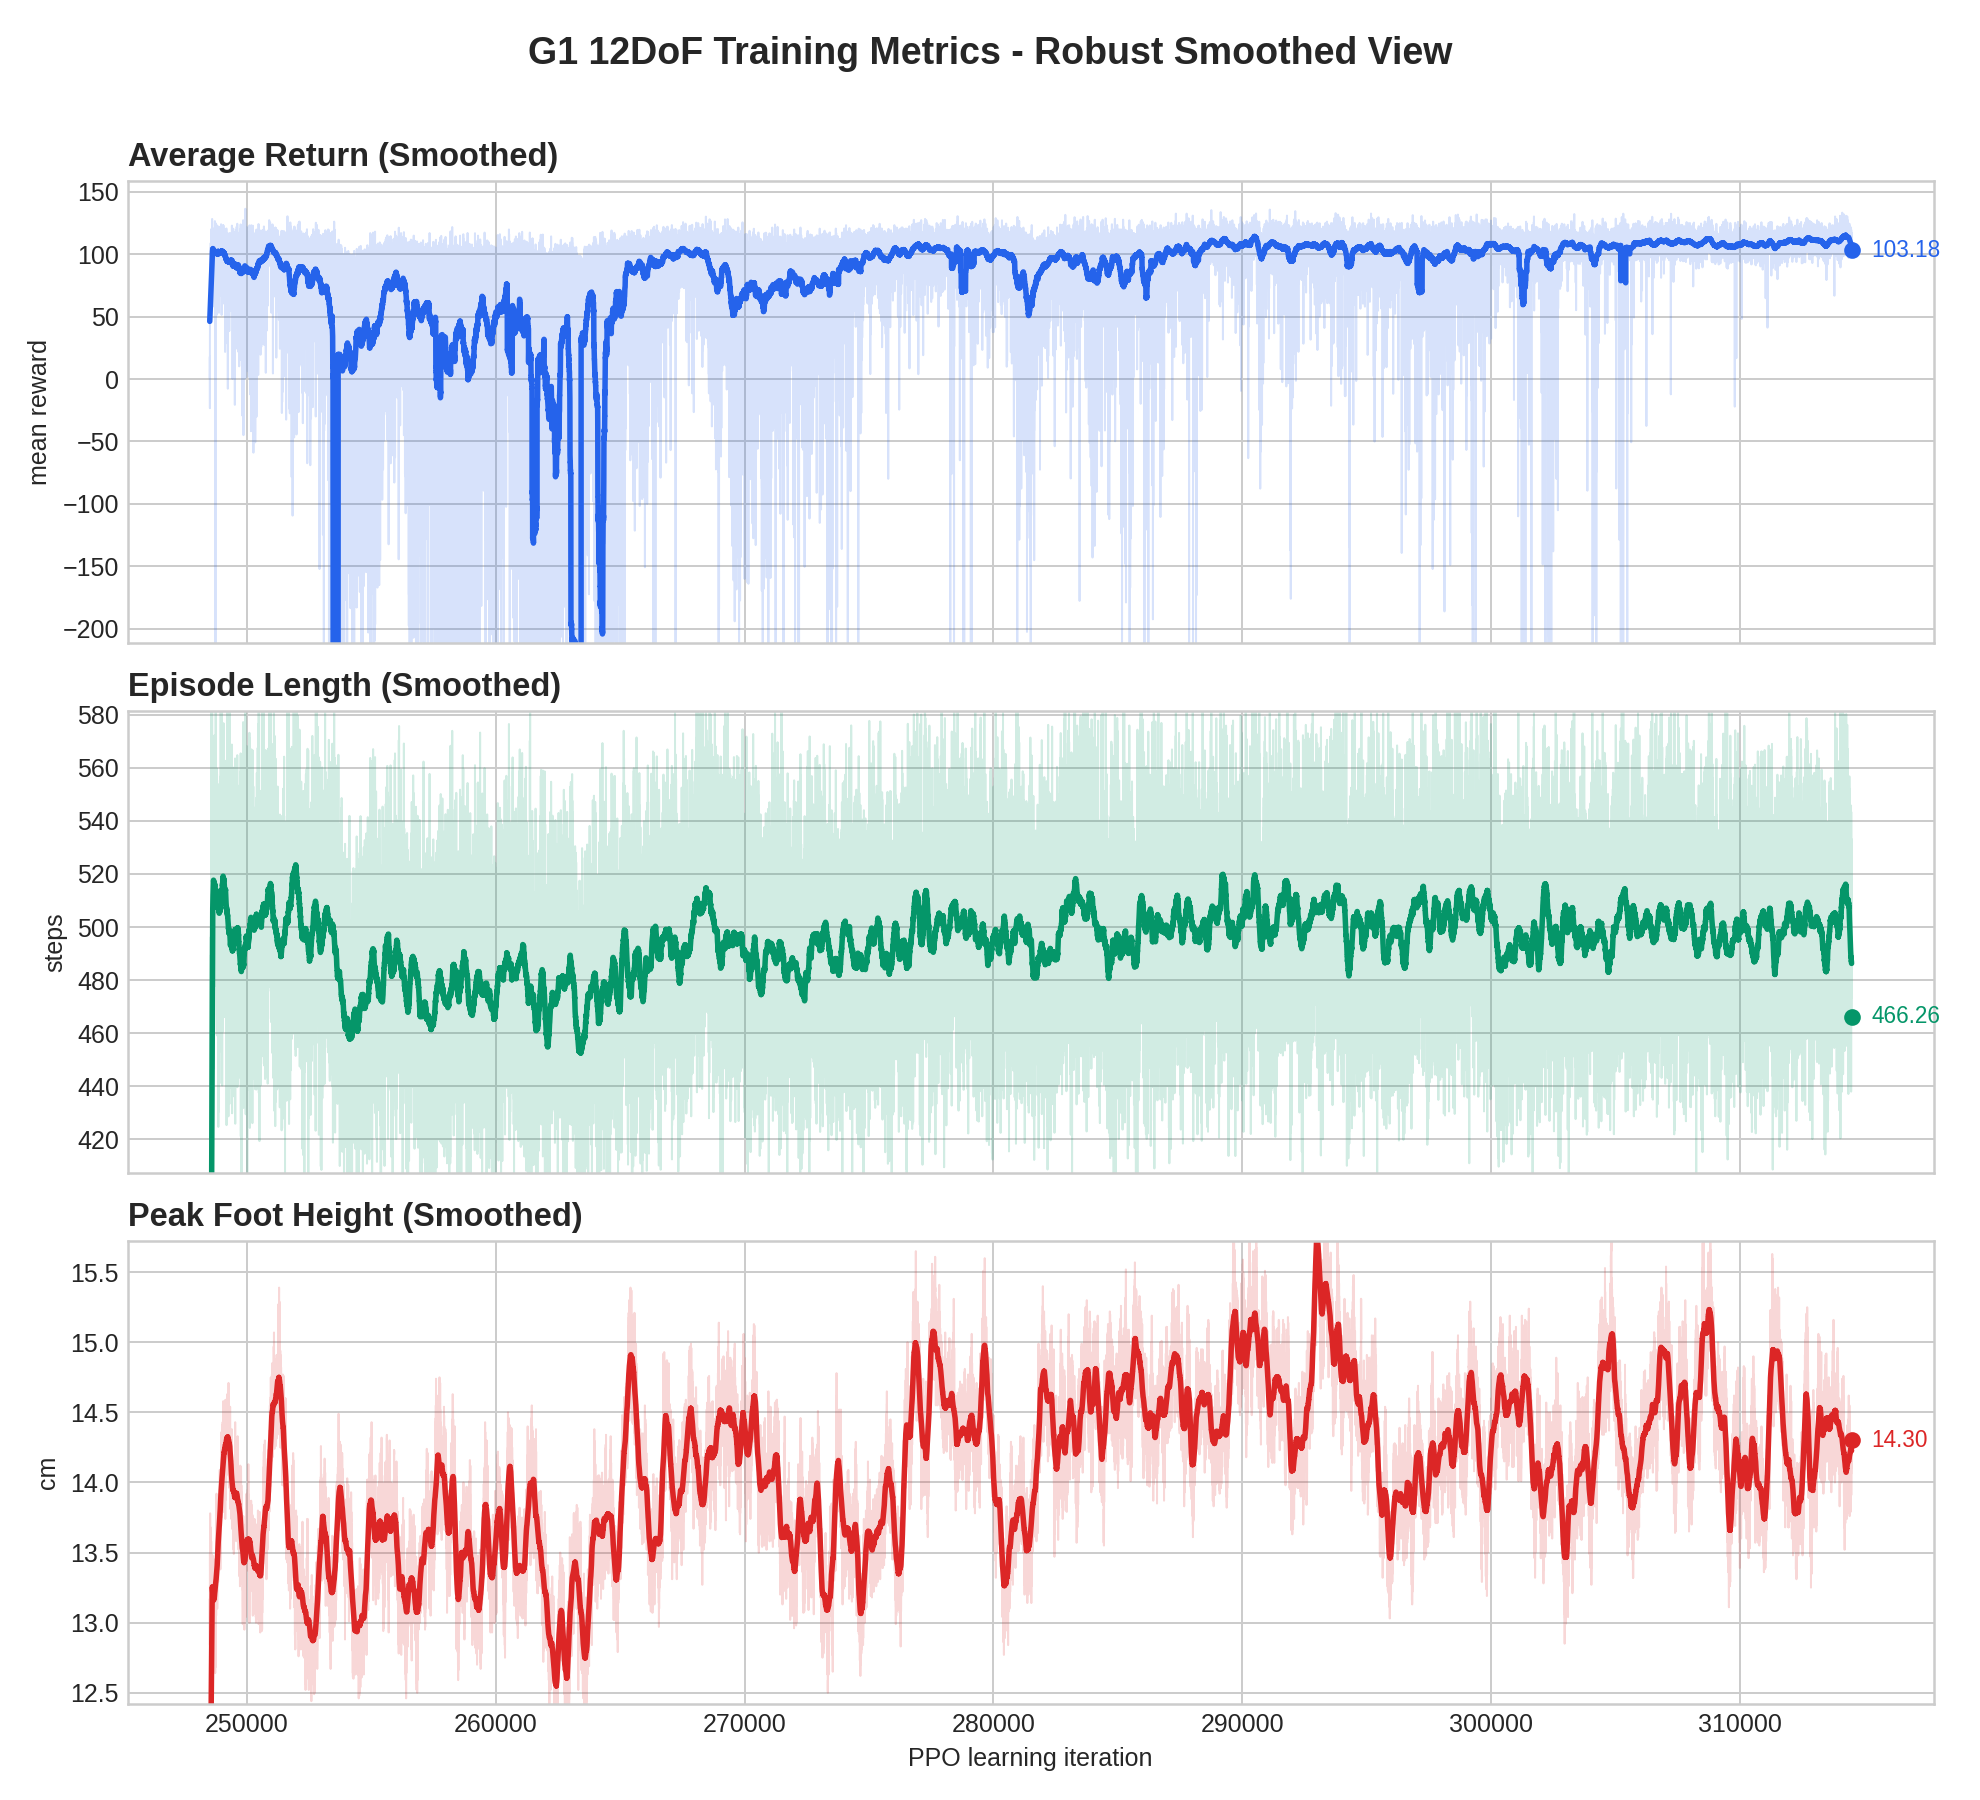
\includegraphics[width=\linewidth]{training_curves_smoothed.png}

    \column{0.33\textwidth}
    \begin{block}{最终阶段指标}
      \begin{itemize}
        \item 平均回报：约 103
        \item 回合长度：约 466 步
        \item 峰值脚高：约 14.3cm
        \item 脚交叉率：0
        \item 双脚同时腾空率：约 1.8\%
      \end{itemize}
    \end{block}

    \begin{block}{解释}
      峰值脚高随训练提升，说明策略逐步获得更强的台阶 clearance；回合长度维持较高，说明未明显训崩。
    \end{block}
  \end{columns}
  \vfill
  {\footnotesize 建议用时：45 秒}
\end{frame}

\begin{frame}{成果展示：交替步态与上下楼梯}
  \begin{columns}[T,onlytextwidth]
    \column{0.50\textwidth}
    \begin{block}{交替迈步}
      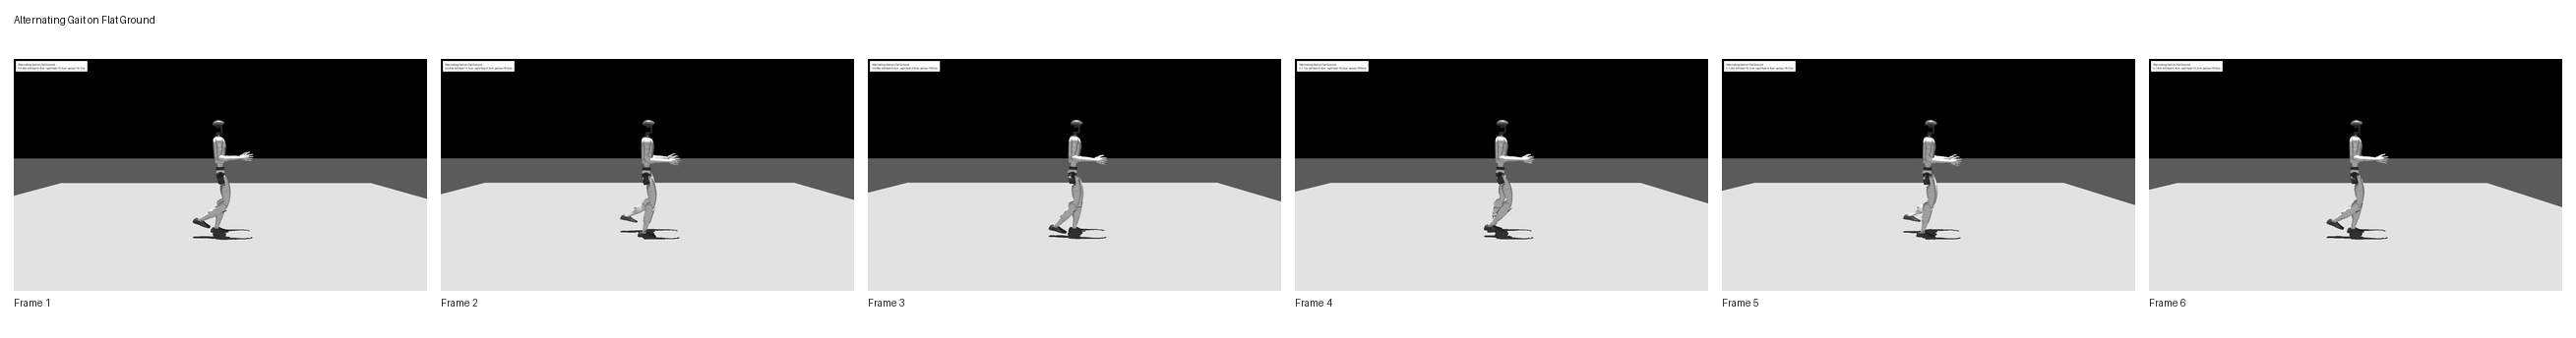
\includegraphics[width=\linewidth]{flat_contact_sheet.png}
    \end{block}
    \vspace{-0.4em}
    {\footnotesize 两脚前后关系周期切换，未出现交叉腿。}

    \column{0.50\textwidth}
    \begin{block}{上楼梯：13.5cm}
      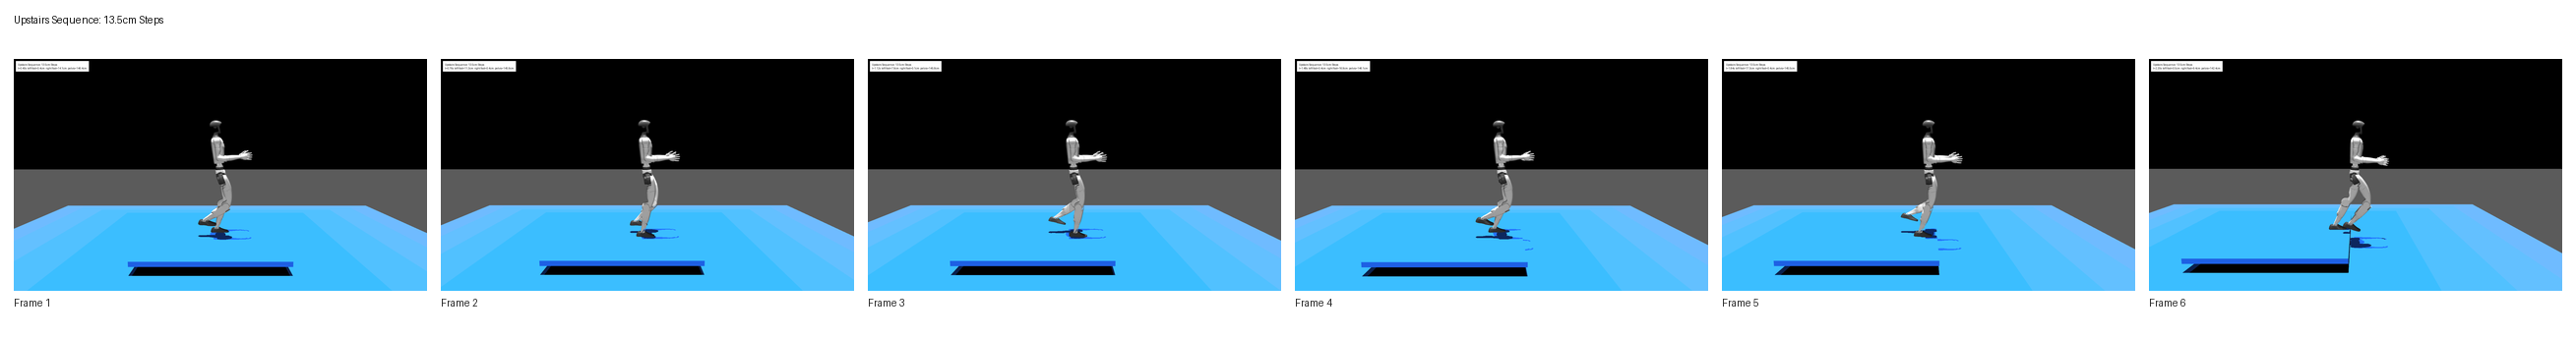
\includegraphics[width=\linewidth]{upstairs_contact_sheet.png}
    \end{block}
    \vspace{-0.4em}
    {\footnotesize 摆动脚抬升跨过台阶，身体保持近似竖直。}
  \end{columns}

  \vspace{0.5em}
  \begin{block}{下楼梯：11.5cm}
    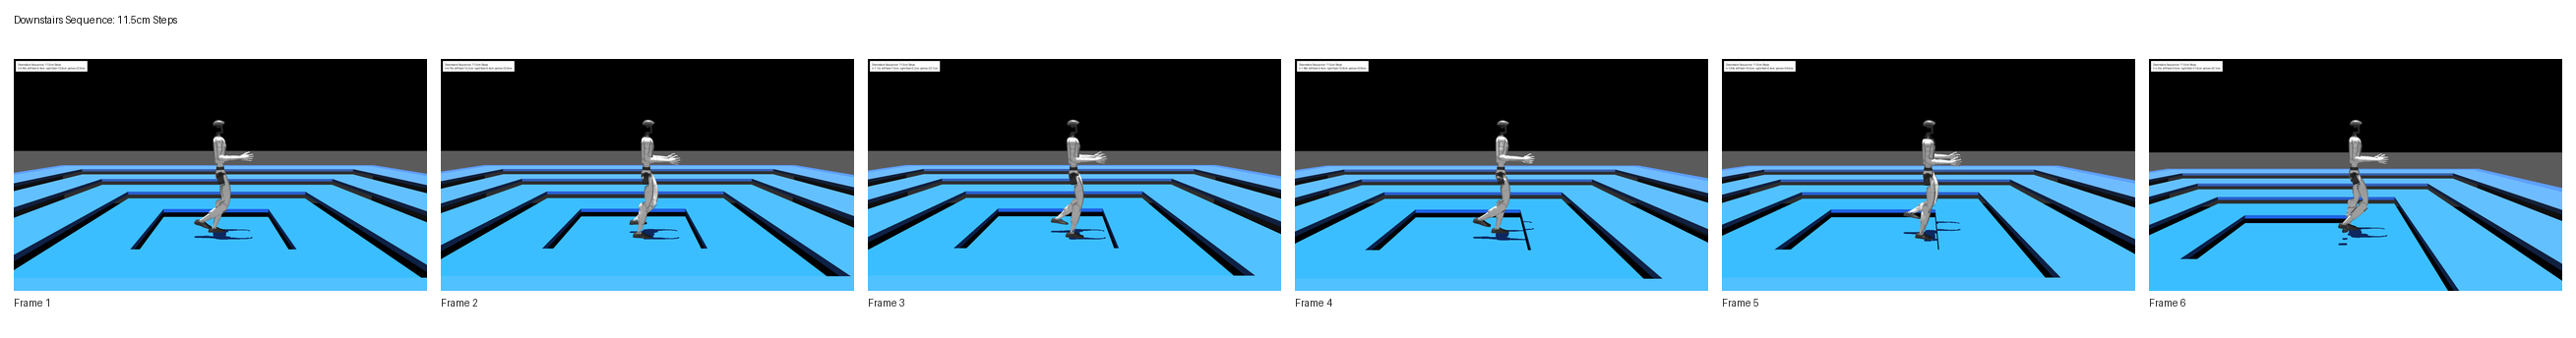
\includegraphics[width=0.92\linewidth]{downstairs_contact_sheet.png}
  \end{block}
  \vfill
  {\footnotesize 建议用时：45 秒}
\end{frame}

\begin{frame}{创新点与后续工作}
  \begin{columns}[T,onlytextwidth]
    \column{0.52\textwidth}
    \begin{block}{创新点}
      \begin{enumerate}
        \item 从“速度奖励”扩展为“步态形态奖励”
        \item 将楼梯高度与脚部 clearance 目标建立几何关系
        \item 使用前后脚顺序切换塑造自然迈步
        \item 课程升级同时检查前进和横向漂移
        \item 训练地形与随机展示地形分离
      \end{enumerate}
    \end{block}

    \column{0.42\textwidth}
    \begin{block}{后续计划}
      \begin{itemize}
        \item 冲击 15cm 台阶
        \item 进一步降低 lateral deviation
        \item 增强右脚抬升稳定性
        \item 加入更真实的物理扰动与硬件迁移约束
      \end{itemize}
    \end{block}

    \begin{alertblock}{核心结论}
      人形感知行走的关键不是让机器人“最快前进”，而是让它用正确的接触相位、足端几何和身体姿态前进。
    \end{alertblock}
  \end{columns}
  \vfill
  {\footnotesize 建议用时：35 秒}
\end{frame}

\begin{frame}{5 分钟时间分配建议}
  \begin{tabular}{llc}
    \toprule
    页码 & 内容 & 时间 \\
    \midrule
    1--2 & 项目概述与汇报结构 & 40s \\
    3--4 & 问题定义与技术路线 & 70s \\
    5--6 & 环境、奖励、训练难点 & 100s \\
    7--8 & 指标与仿真成果 & 90s \\
    9 & 创新点与后续工作 & 35s \\
    10 & 备用页：时间分配 / Q\&A & 余量 \\
    \bottomrule
  \end{tabular}

  \vspace{1em}
  \begin{block}{讲述建议}
    重点不要平均铺开。建议把最多时间放在“为什么普通奖励会训崩”和“我们如何用奖励函数修正步态”两部分。
  \end{block}
\end{frame}

\end{document}
